\documentclass[aps,prb,reprint,nofootinbib]{revtex4-2}

\usepackage{amsmath,amssymb}
\usepackage{graphicx}
\usepackage{booktabs}
\usepackage{listings}
\usepackage{xcolor}

\definecolor{codekw}{HTML}{0072B2}
\definecolor{codestr}{HTML}{009E73}
\definecolor{codecom}{HTML}{777777}

\lstset{
  language=Python,
  basicstyle=\ttfamily\scriptsize,
  keywordstyle=\color{codekw},
  stringstyle=\color{codestr},
  commentstyle=\color{codecom}\itshape,
  numbers=left, numberstyle=\tiny\color{codecom}, numbersep=7pt,
  frame=single, rulecolor=\color{codecom},
  breaklines=true, breakatwhitespace=true,
  showstringspaces=false, tabsize=4,
  columns=fullflexible, keepspaces=true,
  extendedchars=true, inputencoding=utf8,
  literate=%
    {ω}{{$\omega$}}1 {π}{{$\pi$}}1 {μ}{{$\mu$}}1
    {→}{{$\rightarrow$}}1 {≤}{{$\le$}}1 {≥}{{$\ge$}}1
    {—}{{---}}1 {–}{{--}}1 {Δ}{{$\Delta$}}1 {×}{{$\times$}}1
}

\usepackage{hyperref}
\hypersetup{colorlinks=true, linkcolor=black, citecolor=black,
            filecolor=black, urlcolor=blue}

\graphicspath{{../figures/}}

\begin{document}

\title{Phonon Dispersion in a One-Dimensional Multi-atomic Lattice%
\thanks{Solid State Physics, Assignment 1 --- Question 3.}}

\author{Guhan Dhanasekharan\,\,(EP24BTECH11011)}
\author{Kumud Jalori\,\,(EP24BTECH11015)}
\author{Naman Verma\,\,(EP24BTECH11016)}
\author{Nazakar Abhilash\,\,(EP24BTECH11017)}
\author{Nithin Surya S\,\,(EP24BTECH11018)}
\author{Panduru Sri Abish\,\,(EP24BTECH11019)}
\author{Prasang Das\,\,(EP24BTECH11020)}
\author{Praveen Kumar\,\,(EP24BTECH11021)}
\author{S Haresh\,\,(EP24BTECH11022)}
\author{S Kshiteesh\,\,(EP24BTECH11023)}
\affiliation{Department of Engineering Physics}

\date{\today}

\begin{abstract}
We compute the phonon dispersion of a one-dimensional lattice carrying $p$ atoms of arbitrary
mass per unit cell, coupled by nearest-neighbour springs. The equations of motion are reduced by
a Bloch ansatz to a $p \times p$ Hermitian eigenvalue problem, which we diagonalise numerically
across the first Brillouin zone. The method is validated against the closed-form monatomic and
diatomic solutions, reproducing them to $4 \times 10^{-14}$. An interactive interface built with
Streamlit exposes $p$, the masses, the spring constant and the lattice constant, and reports the
acoustic and optical branches, their frequency limits, the bandgaps between them, and the
eigenfrequencies at the zone centre and edge. Three parameter sets demonstrate that the gap is
controlled by mass contrast and closes entirely when the masses are equal, while the spring
constant sets the overall frequency scale as $\sqrt{K}$ without altering the shape of the
spectrum.
\end{abstract}

\maketitle

\section{Introduction}

A crystal at finite temperature is not a static array of atoms: each atom oscillates about its
equilibrium site, and because the atoms are coupled, those oscillations propagate as waves. The
quantised normal modes of these waves are phonons, and the relation $\omega(q)$ between a mode's
frequency and its wavevector --- the dispersion relation --- governs the solid's heat capacity,
thermal conductivity and sound velocity.

The one-dimensional chain is the standard setting for this problem because it is exactly solvable
and still contains the essential physics. A chain with one atom per cell supports a single
\emph{acoustic} branch. Placing $p$ atoms in the cell produces $p$ branches: one acoustic and
$p-1$ \emph{optical}. Where the masses differ, a frequency gap opens between them, inside which
no travelling wave exists at any wavevector.

This report derives the general $p$-atom dispersion relation, implements it, validates it against
the cases that can be solved by hand, and uses it to examine how masses and spring constants
control the spectrum.

\section{Theory}
\label{sec:theory}

\subsection{Equations of motion}

\begin{figure*}[t]
\centering
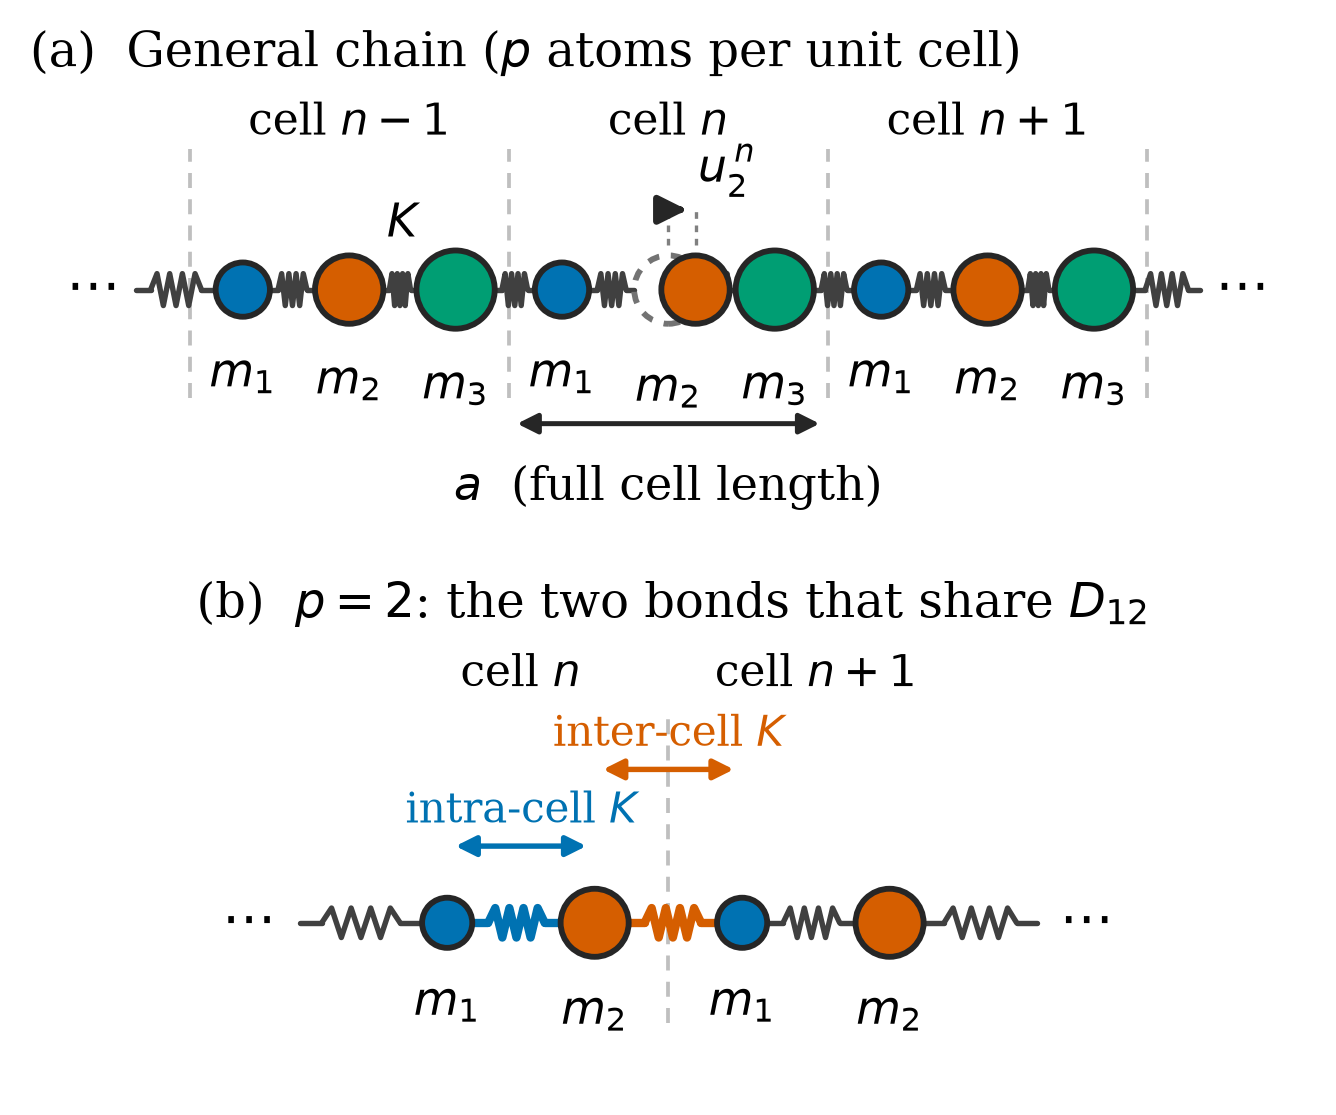
\includegraphics[width=0.60\textwidth]{schematic.png}
\caption{The model. (a) Three unit cells of the general $p$-atom chain; circle area scales with
mass, $a$ is the full cell length, and $u_2^{\,n}$ marks a longitudinal displacement from the
equilibrium site (dashed). (b) The $p=2$ case. Both bonds join the same pair $m_1$--$m_2$, one
inside cell $n$ and one across the boundary, so both land in the same matrix element $D_{12}$
and the implementation must \emph{accumulate} their contributions rather than overwrite one with
the other --- see Sec.~\ref{sec:theory}.}
\label{fig:schematic}
\end{figure*}

Consider a chain of identical unit cells of length $a$, as in Fig.~\ref{fig:schematic}(a).
Cell $n$ contains $p$ atoms of masses $m_1, \dots, m_p$. Let $u_j^n$ be the displacement of atom $j$ in cell $n$ from its equilibrium
position. Nearest neighbours are joined by springs of constant $K$, so in the harmonic
approximation the force on an atom is linear in the \emph{relative} displacements of its two
neighbours:
\begin{equation}
  m_j \ddot{u}_j^{\,n} = K\left(u_{j+1}^{\,n} - u_j^{\,n}\right)
                        + K\left(u_{j-1}^{\,n} - u_j^{\,n}\right).
  \label{eq:eom}
\end{equation}
The chain is closed by the identifications $u_{p+1}^{\,n} \equiv u_1^{\,n+1}$ and
$u_0^{\,n} \equiv u_p^{\,n-1}$: the last atom of a cell bonds to the first atom of the next.
Equation~\eqref{eq:eom} is a coupled system of infinitely many ordinary differential equations,
one per atom.

\subsection{Bloch ansatz and the dynamical matrix}

The system is invariant under translation by $a$, so by Bloch's theorem the solutions are plane
waves modulated by a cell-periodic amplitude. We take
\begin{equation}
  u_j^{\,n} = \frac{1}{\sqrt{m_j}}\, e_j \, e^{i(qna - \omega t)},
  \label{eq:bloch}
\end{equation}
where the factor $m_j^{-1/2}$ is a choice, not a restriction: it makes the resulting matrix
Hermitian rather than merely similar to a Hermitian matrix, which is what allows a stable
eigensolver to be used below.

Substituting \eqref{eq:bloch} into \eqref{eq:eom} and cancelling the common exponential turns the
infinite system into a finite $p \times p$ eigenvalue problem,
\begin{equation}
  D(q)\, \mathbf{e} = \omega^2 \mathbf{e},
  \label{eq:eigen}
\end{equation}
with the \emph{mass-weighted dynamical matrix}
\begin{align}
  D_{jj}     &= \frac{2K}{m_j}, \label{eq:Ddiag}\\
  D_{j,j+1} = D_{j+1,j} &= -\frac{K}{\sqrt{m_j m_{j+1}}}, \qquad j = 1,\dots,p-1, \label{eq:Dintra}\\
  D_{1,p}    &= -\frac{K\,e^{-iqa}}{\sqrt{m_1 m_p}}, \qquad D_{p,1} = D_{1,p}^{*}. \label{eq:Dinter}
\end{align}
Only the inter-cell element \eqref{eq:Dinter} depends on $q$; the phase $e^{-iqa}$ is the
Bloch factor picked up on crossing a cell boundary. Since $D(q)^\dagger = D(q)$, its eigenvalues
$\omega^2$ are real, and since the harmonic lattice is mechanically stable they are
non-negative.

\paragraph{A caution on conventions.} Here $a$ is the \emph{full unit-cell length}. Many texts
treating the diatomic chain set $a$ to the nearest-neighbour spacing, making the cell $2a$ long;
their $\cos(qa)$ is our $\cos(qa/2)$. Mixing the two conventions introduces a silent factor of
two into every plotted frequency. All results below use the full-cell convention.

\paragraph{A caution on the $p=2$ case.} When the cell holds exactly two atoms, the intra-cell
bond \eqref{eq:Dintra} and the inter-cell bond \eqref{eq:Dinter} occupy the \emph{same} matrix
element, as Fig.~\ref{fig:schematic}(b) shows: atom 1 bonds to atom 2 twice, once inside the cell and once across the boundary. The two
contributions must therefore be added, giving
$D_{12} = -K\left(1 + e^{-iqa}\right)/\sqrt{m_1 m_2}$. Overwriting rather than accumulating is an
easy implementation error, and it breaks the physics: the acoustic branch no longer vanishes at
$q=0$, violating translational invariance.

\subsection{Branch structure}

Diagonalising \eqref{eq:eigen} at each $q$ in the first Brillouin zone, $q \in [-\pi/a, \pi/a]$,
gives $p$ frequencies. Ordering them ascending at every $q$:

\begin{itemize}
  \item the lowest, $\omega_1(q)$, is the \textbf{acoustic} branch. It satisfies
        $\omega_1(0)=0$, because a uniform translation of the entire crystal costs no energy ---
        this is a direct consequence of $D(0)$ having a null vector $e_j \propto \sqrt{m_j}$.
        Near $q=0$ it is linear, $\omega_1 \simeq v_s |q|$, with
        \begin{equation}
          v_s = a\sqrt{\frac{K}{p\sum_j m_j}},
          \label{eq:vs}
        \end{equation}
        obtained by treating the cell as $p$ springs in series over a length $a$ carrying total
        mass $\sum_j m_j$. This is the speed of sound in the chain.
  \item the remaining $p-1$ branches are \textbf{optical}. They stay finite as $q \to 0$, where
        they describe the atoms within a cell oscillating against one another with the cell's
        centre of mass at rest.
\end{itemize}

\subsection{Closed forms used for validation}

For $p=1$ (mass $m$) the matrix is $1\times1$ and
\begin{equation}
  \omega(q) = 2\sqrt{\frac{K}{m}}\left|\sin\frac{qa}{2}\right|.
  \label{eq:mono}
\end{equation}
For $p=2$ (masses $m_1, m_2$) the $2\times2$ determinant gives, writing
$\mu^{-1} \equiv m_1^{-1} + m_2^{-1}$ for the reduced mass,
\begin{equation}
  \omega_\pm^2 = \frac{K}{\mu}
    \pm K \left[\frac{1}{\mu^2} - \frac{4\sin^2(qa/2)}{m_1 m_2}\right]^{1/2},
  \label{eq:di}
\end{equation}
with $\omega_-$ acoustic and $\omega_+$ optical. At the zone boundary these reduce to
$\omega_- = \sqrt{2K/m_{>}}$ and $\omega_+ = \sqrt{2K/m_{<}}$, where $m_{>}$ and $m_{<}$ are the
larger and smaller mass --- so the gap at the zone edge is set purely by the mass contrast and
vanishes when $m_1 = m_2$.

\section{Numerical method}

The procedure is deliberately direct; no iteration or convergence criterion is involved.

\begin{enumerate}
  \item Build a grid of $n_q$ wavevectors spanning the first Brillouin zone.
  \item At each $q$, assemble $D(q)$ from \eqref{eq:Ddiag}--\eqref{eq:Dinter} as a complex
        $p \times p$ array, accumulating the inter-cell bond as noted above.
  \item Diagonalise with \texttt{numpy.linalg.eigvalsh}, the solver for Hermitian matrices. It
        returns real eigenvalues in ascending order, which is exactly the branch ordering we
        want, so no sorting step is needed.
  \item Take $\omega = \sqrt{\omega^2}$, clipping values at zero first: at $q=0$ the acoustic
        eigenvalue is zero up to rounding and can emerge as a small negative number, whose square
        root would be \texttt{nan}.
  \item Extract the per-branch minima and maxima, and identify a gap between branches $i$ and
        $i+1$ whenever $\min_q \omega_{i+1} > \max_q \omega_i$.
\end{enumerate}

The cost is $n_q$ diagonalisations of a $p \times p$ matrix, negligible for the sizes here, which
is why the interface can recompute the full spectrum on every slider movement.

The whole of the physics is the assembly in step 2 together with the single call in step 3; the
rest of the codebase computes derived quantities, validates them, or draws them.
Listing~\ref{lst:core} is the implementation, reproduced verbatim from
\texttt{phonon.py}.

\begin{lstlisting}[caption={Construction of the dynamical matrix. The \texttt{+=} on the
inter-cell bond is the subtlety discussed in Sec.~\ref{sec:theory}.},label={lst:core},
firstnumber=1]
D = np.zeros((p, p), dtype=complex)
np.fill_diagonal(D, 2.0 * K / m)

# intra-cell bonds
for j in range(p - 1):
    c = -K / np.sqrt(m[j] * m[j + 1])
    D[j, j + 1] = c
    D[j + 1, j] = c

# inter-cell bond, carries all the q-dependence
c = -K * np.exp(-1j * q * a) / np.sqrt(m[0] * m[-1])
D[0, -1] += c
D[-1, 0] += np.conj(c)

# D is Hermitian, so eigvalsh gives real, ascending eigenvalues
w2 = np.linalg.eigvalsh(D)
omega = np.sqrt(np.clip(w2, 0.0, None))
\end{lstlisting}

\subsection{Validation}

Five checks run in \texttt{test\_phonon.py}; all pass.

\begin{table*}[t]
\centering
\small
\begin{tabular}{llr}
\toprule
\textbf{Check} & \textbf{What it tests} & \textbf{Result} \\
\midrule
Diatomic vs Eq.~\eqref{eq:di}    & the general code in the solvable case   & $4.5\times10^{-14}$ \\
Monatomic vs Eq.~\eqref{eq:mono} & the $p=1$ wrap-around branch            & $1.6\times10^{-15}$ \\
Zone folding                     & equal masses in a $3a$ cell unfold onto Eq.~\eqref{eq:mono} & $1.4\times10^{-4}$ \\
Sound velocity                   & $q\to0$ slope against Eq.~\eqref{eq:vs} & $1.6\times10^{-8}$ \\
$\omega_1(0)=0$                  & translational invariance                & $0$ exactly \\
Gap closure                      & equal masses leave no gap               & pass \\
\bottomrule
\end{tabular}
\caption{Validation results. The first two columns are maximum absolute errors over the zone; the
zone-folding figure is limited by the finite $q$ grid, not by the method.}
\end{table*}

Figure~\ref{fig:validation} shows the diatomic check graphically: the numerically obtained points
lie on the analytic curves everywhere in the zone.

\begin{figure}[h]
\centering
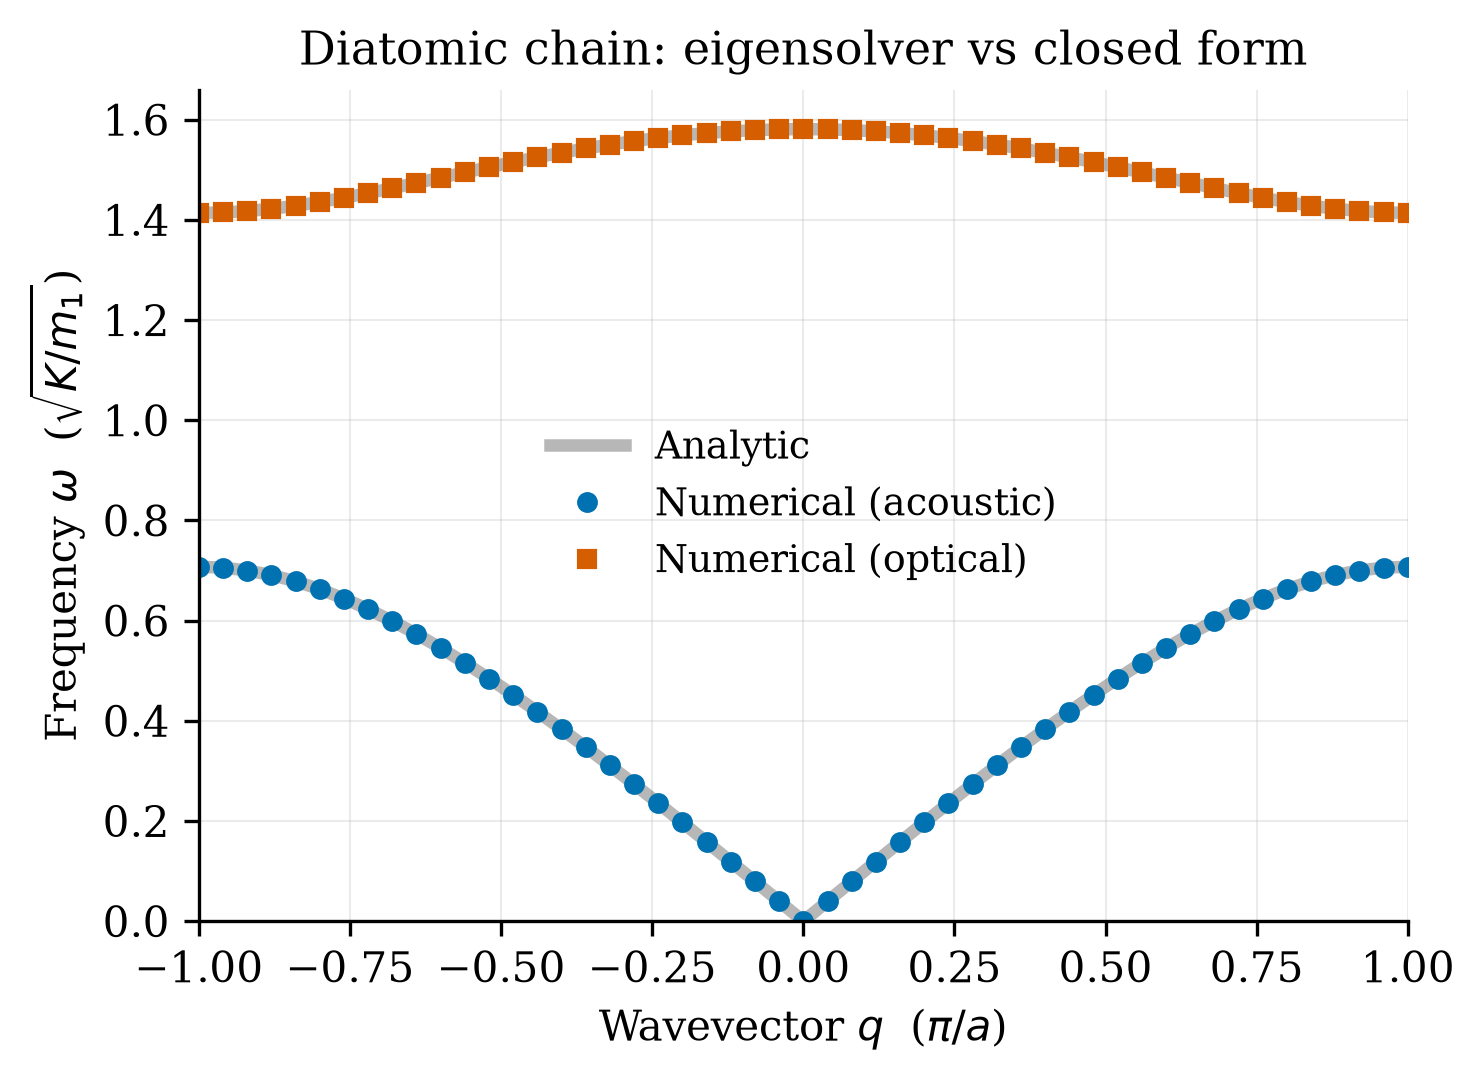
\includegraphics[width=\columnwidth]{validation.png}
\caption{Numerical eigenfrequencies (markers) against the closed-form diatomic solution
Eq.~\eqref{eq:di} (grey), for $m=(1,4)$, $K=1$.}
\label{fig:validation}
\end{figure}

\section{The interactive interface}

The interface is written with Streamlit and launched with \texttt{streamlit run app.py}. The
sidebar accepts the number of atoms per cell $p$, one mass field per atom, the spring constant
$K$, the lattice constant $a$, and the $q$-grid density; three presets load the demonstration
cases below. Every change triggers a recomputation.

The main panel shows the dispersion with the acoustic branch drawn separately from the optical
ones, each gap shaded across the zone and annotated with its width, and tables giving the
frequency limits of every branch, every bandgap, the analytic sound velocity, and the
eigenfrequencies at $q=0$ and $q=\pi/a$. The density of states is plotted underneath.

Figures~\ref{fig:ui} and \ref{fig:ui2} show the interface running on two of the demonstration cases. Switching
preset from the diatomic Case A to the triatomic Case C changes the number of mass fields, adds
a third branch to the plot, and produces a second bandgap row in the table --- all from the same
code path, with no special-casing for the number of atoms per cell. The values displayed agree
with Tables~\ref{tab:cases} and \ref{tab:eigen} to the digits shown.

\begin{figure*}[t]
\centering
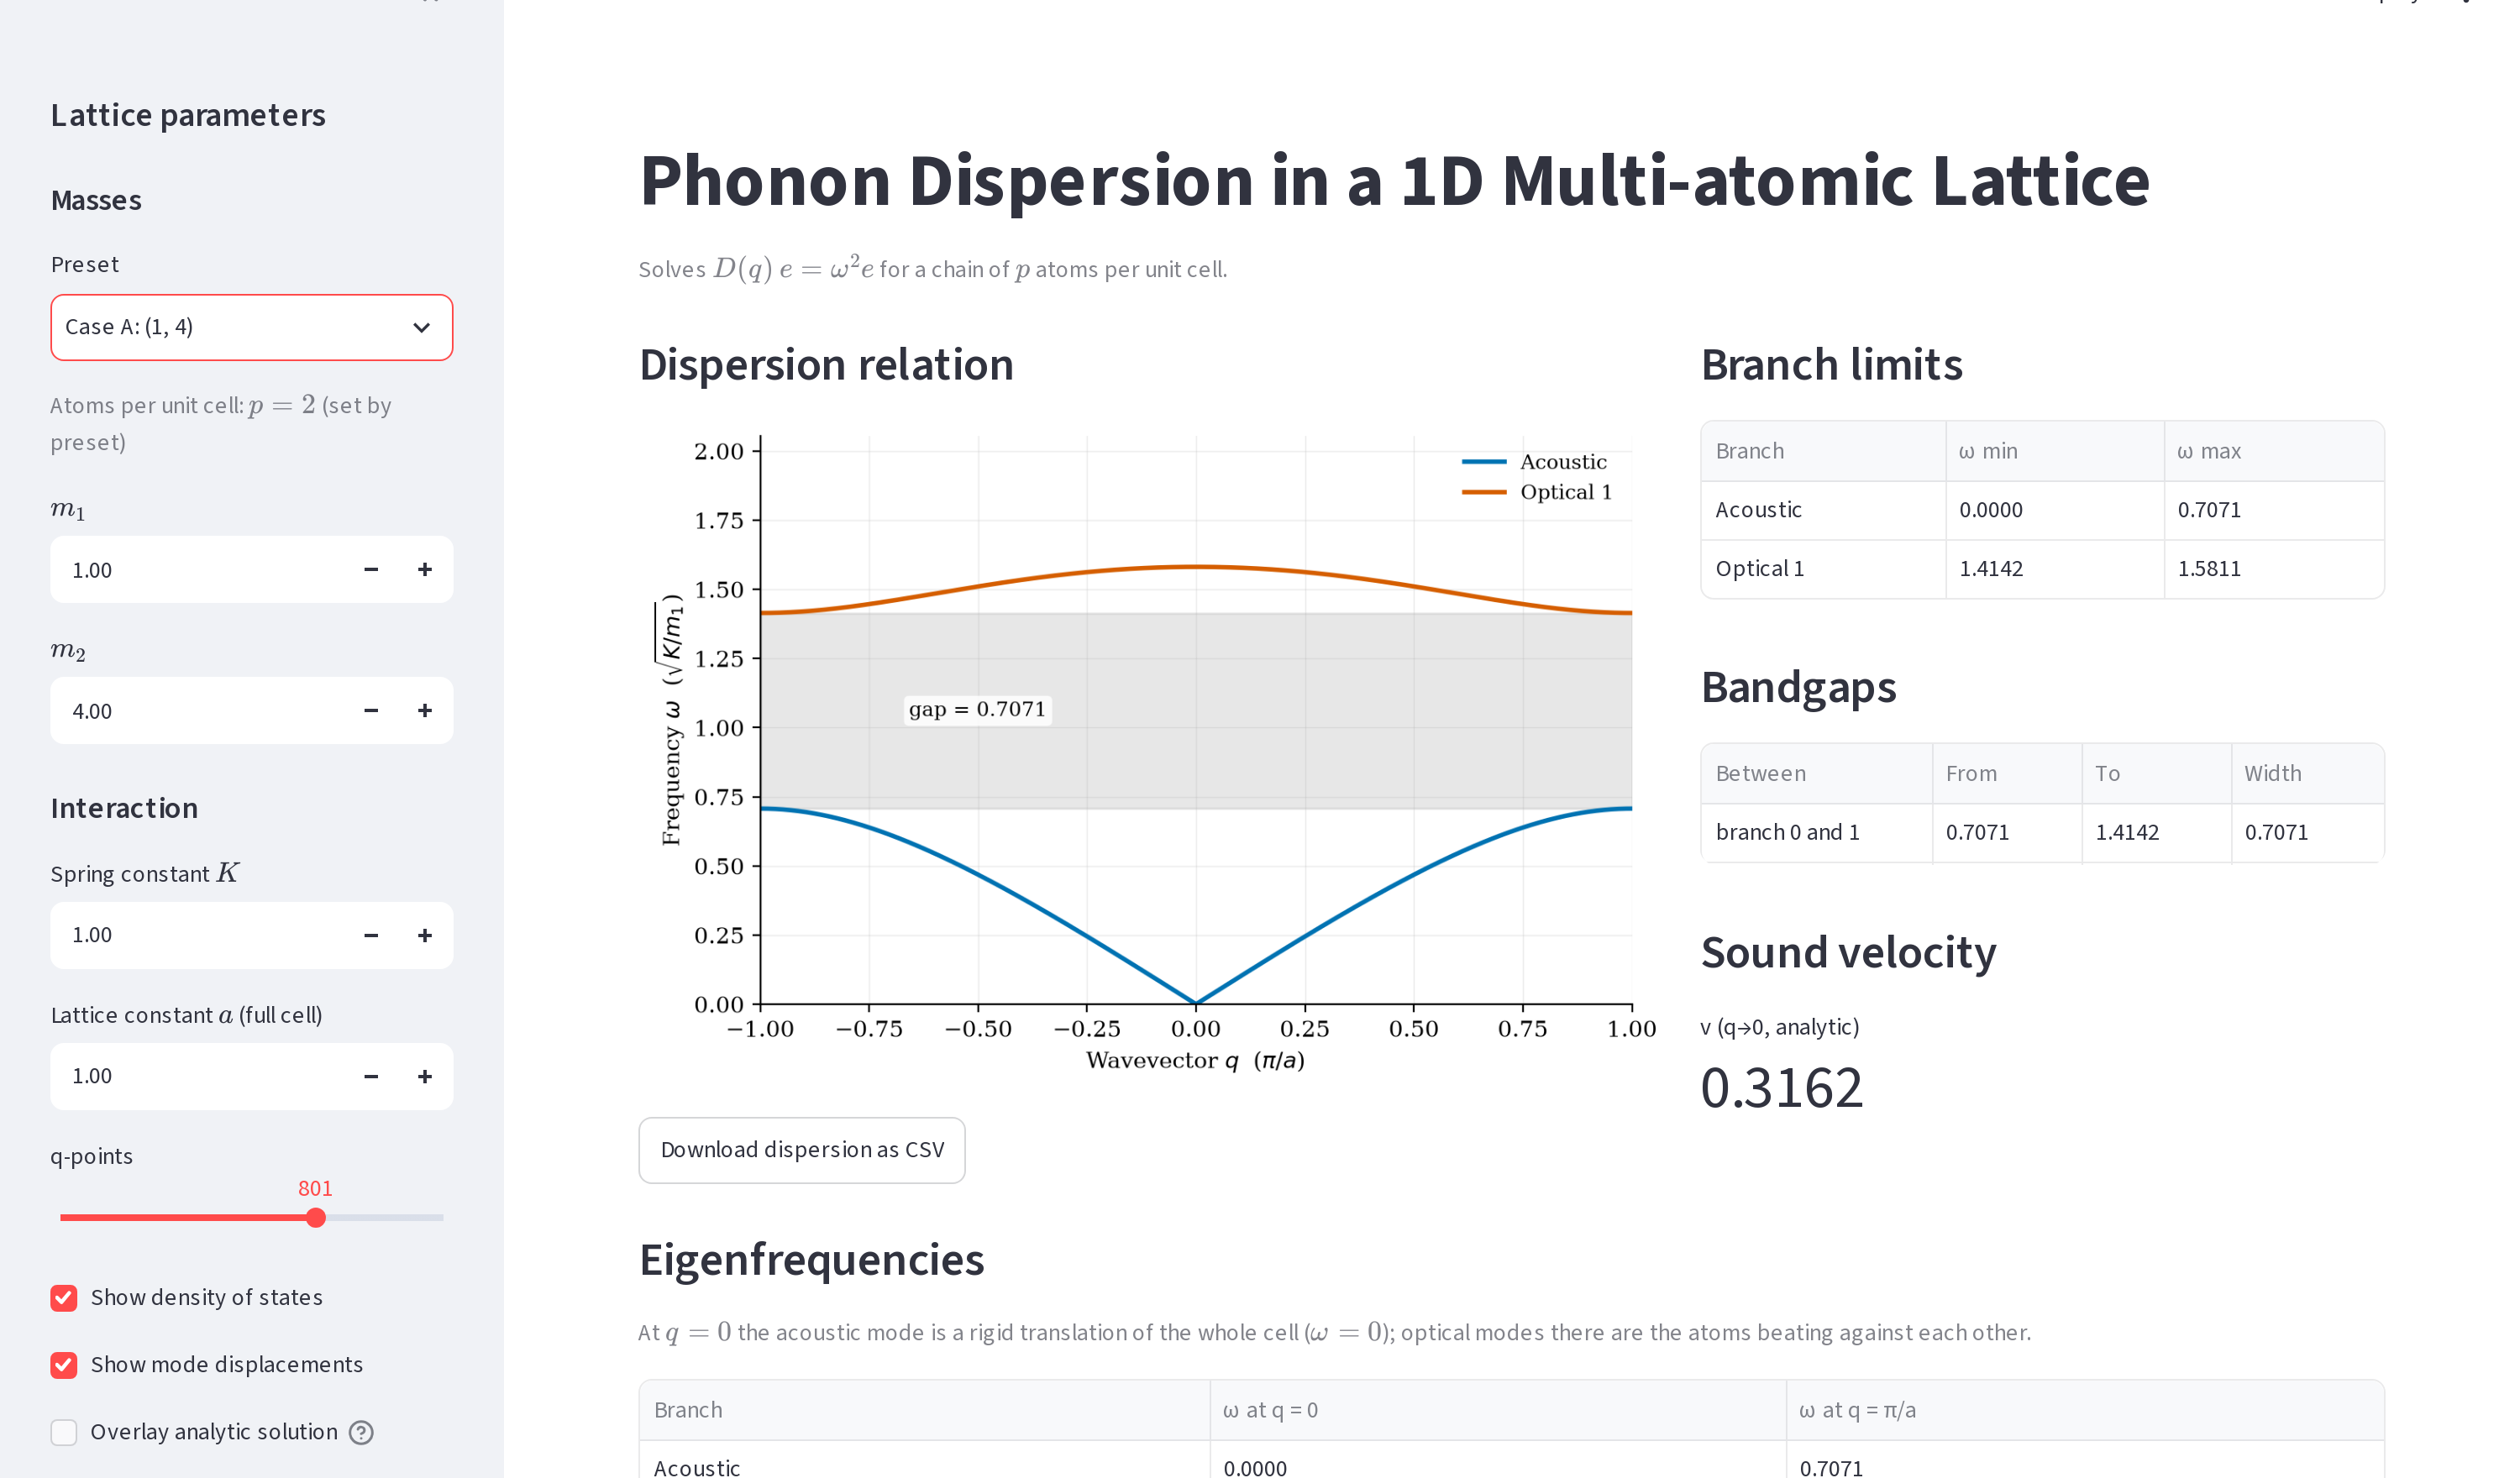
\includegraphics[width=0.92\textwidth]{ui_case_a_top.png}
\caption{The interface on Case A ($p=2$). The sidebar carries the lattice parameters; the main
panel gives the dispersion with the bandgap shaded and annotated, the per-branch frequency
limits, every bandgap, the analytic sound velocity, and the zone-centre and zone-edge
eigenfrequencies. Density-of-states and mode-displacement panels continue below the region
shown.}
\label{fig:ui}
\end{figure*}

\begin{figure*}[t]
\centering
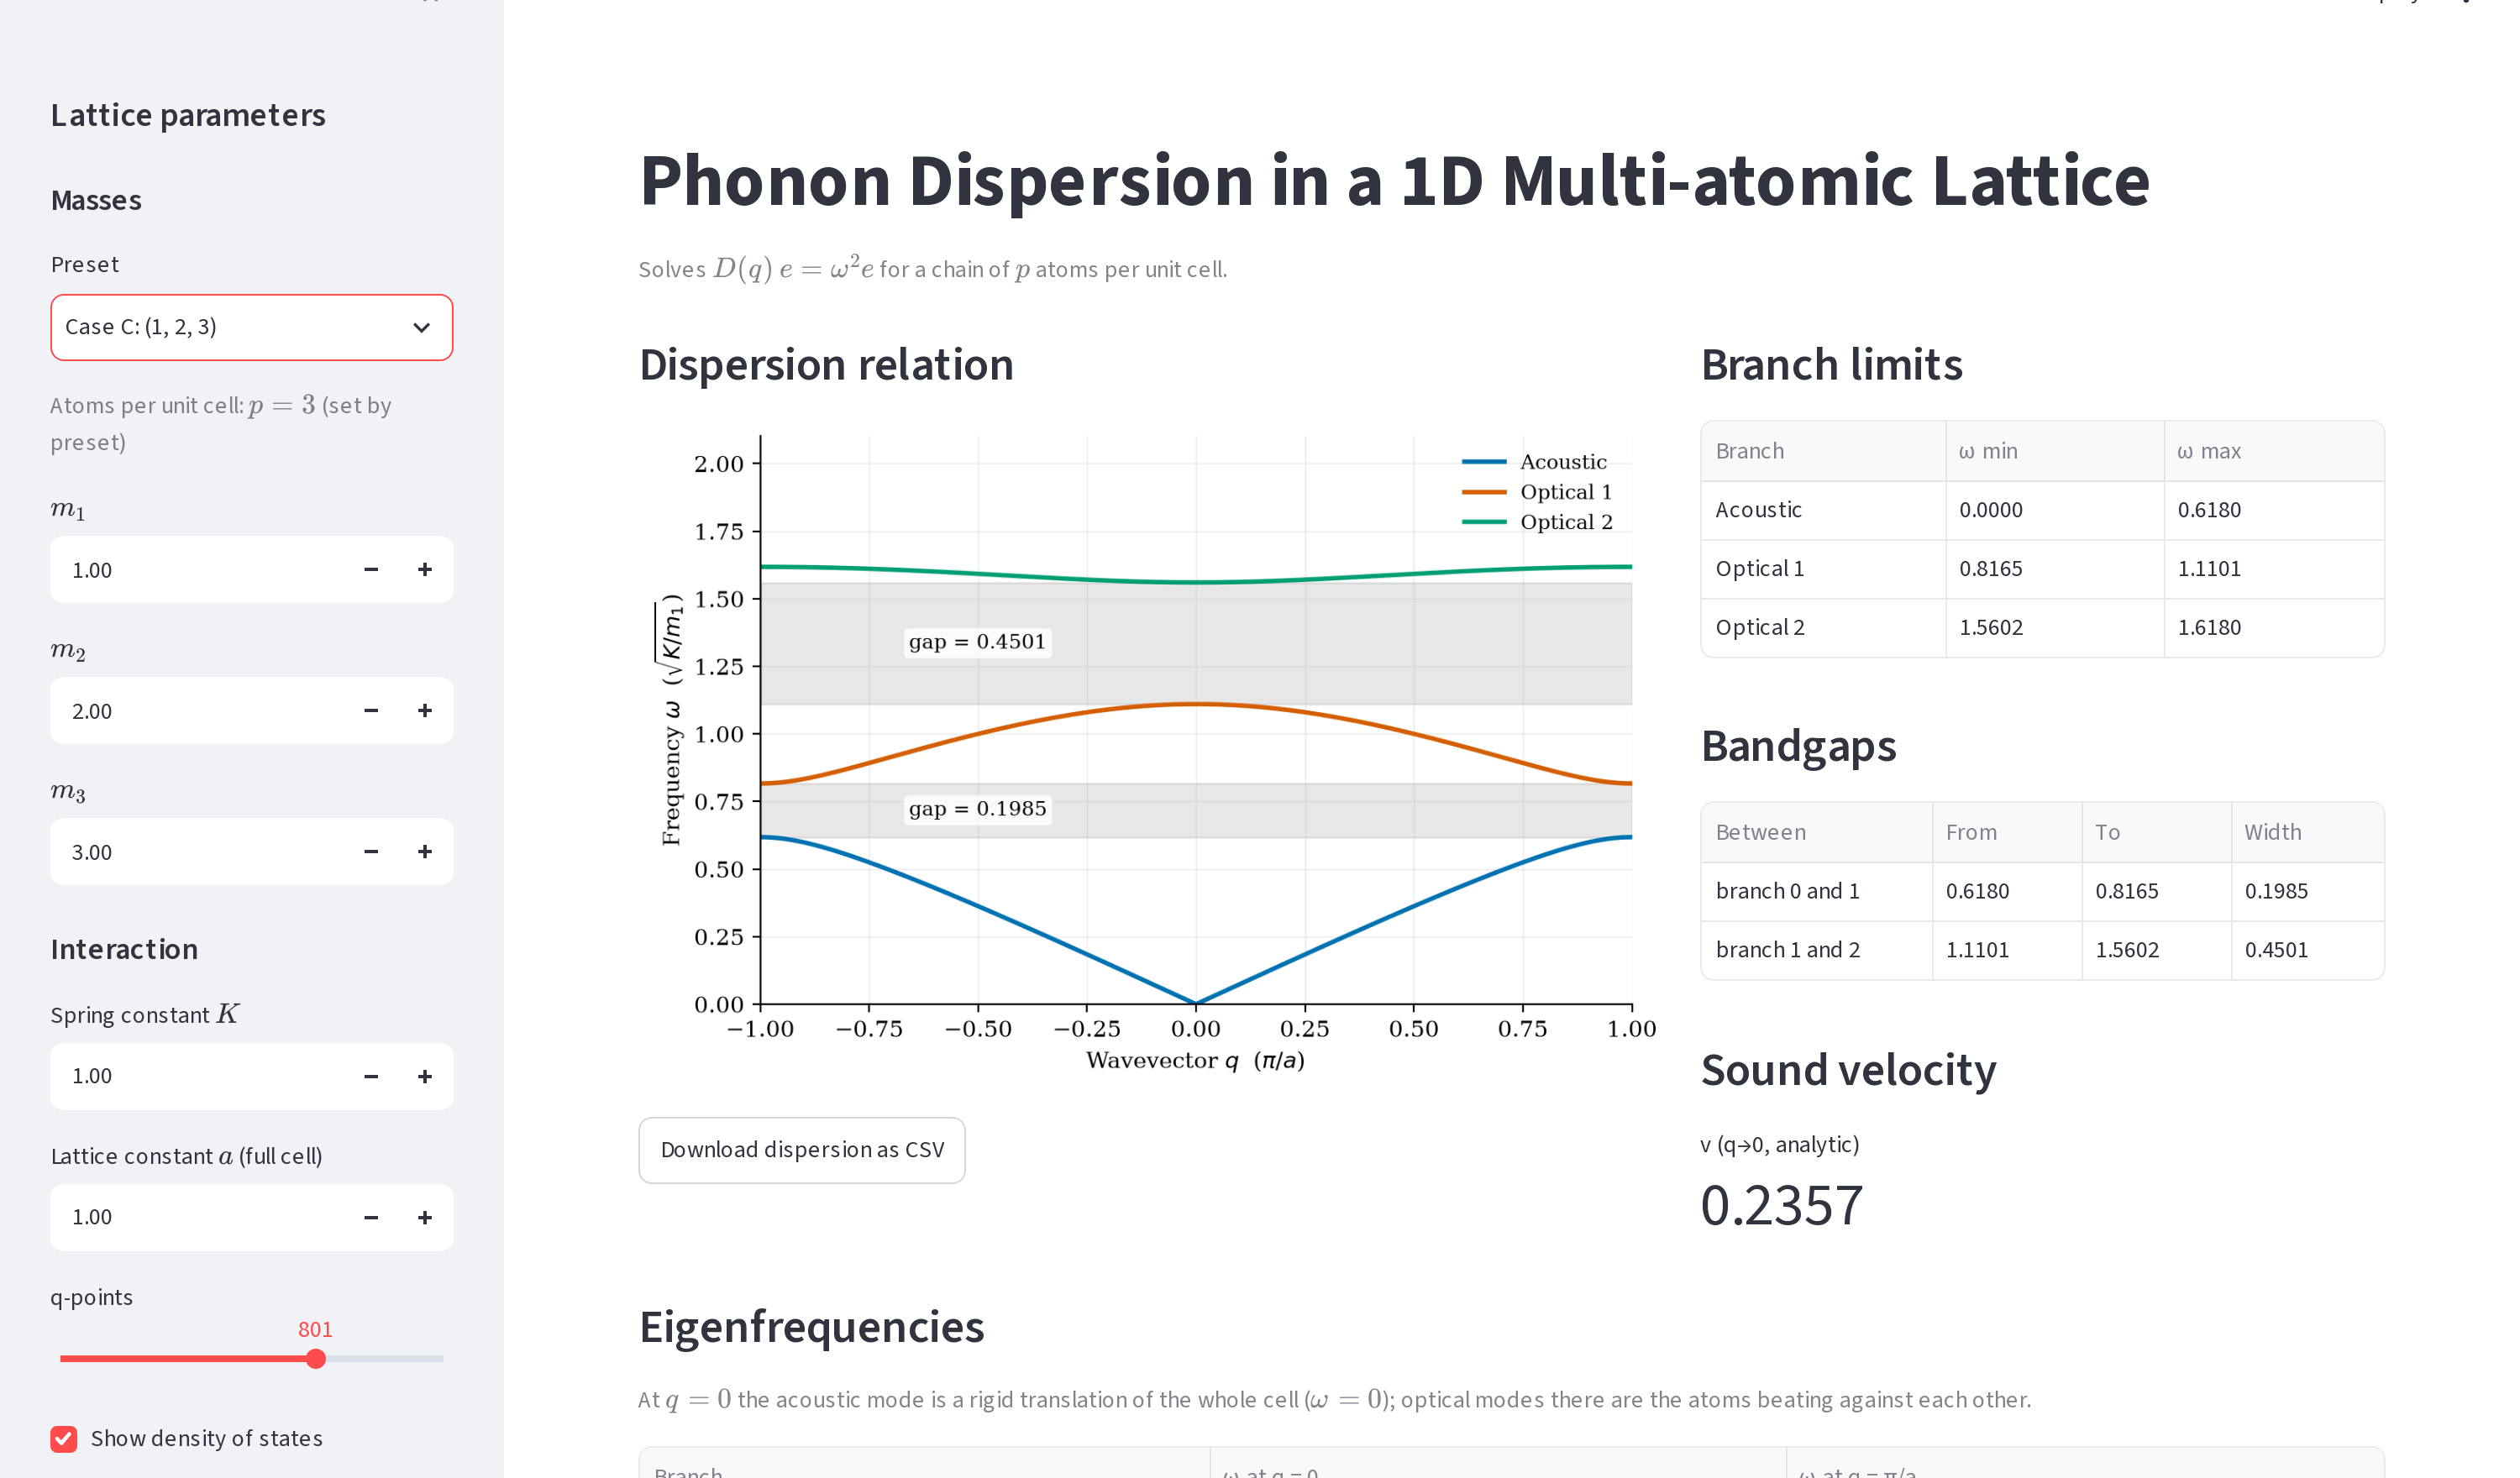
\includegraphics[width=0.92\textwidth]{ui_case_c_top.png}
\caption{The same interface on Case C ($p=3$). Selecting the preset adds a third mass field, a
third branch, and a second row to the bandgap table, with no change of code path. The displayed
values match Tables~\ref{tab:cases} and \ref{tab:eigen}.}
\label{fig:ui2}
\end{figure*}

\section{Results}

All results use $K=1$, $a=1$ and quote frequencies in units of $\sqrt{K/m_1}$. Three
mass/spring combinations are compared.

\begin{figure*}[t]
\centering
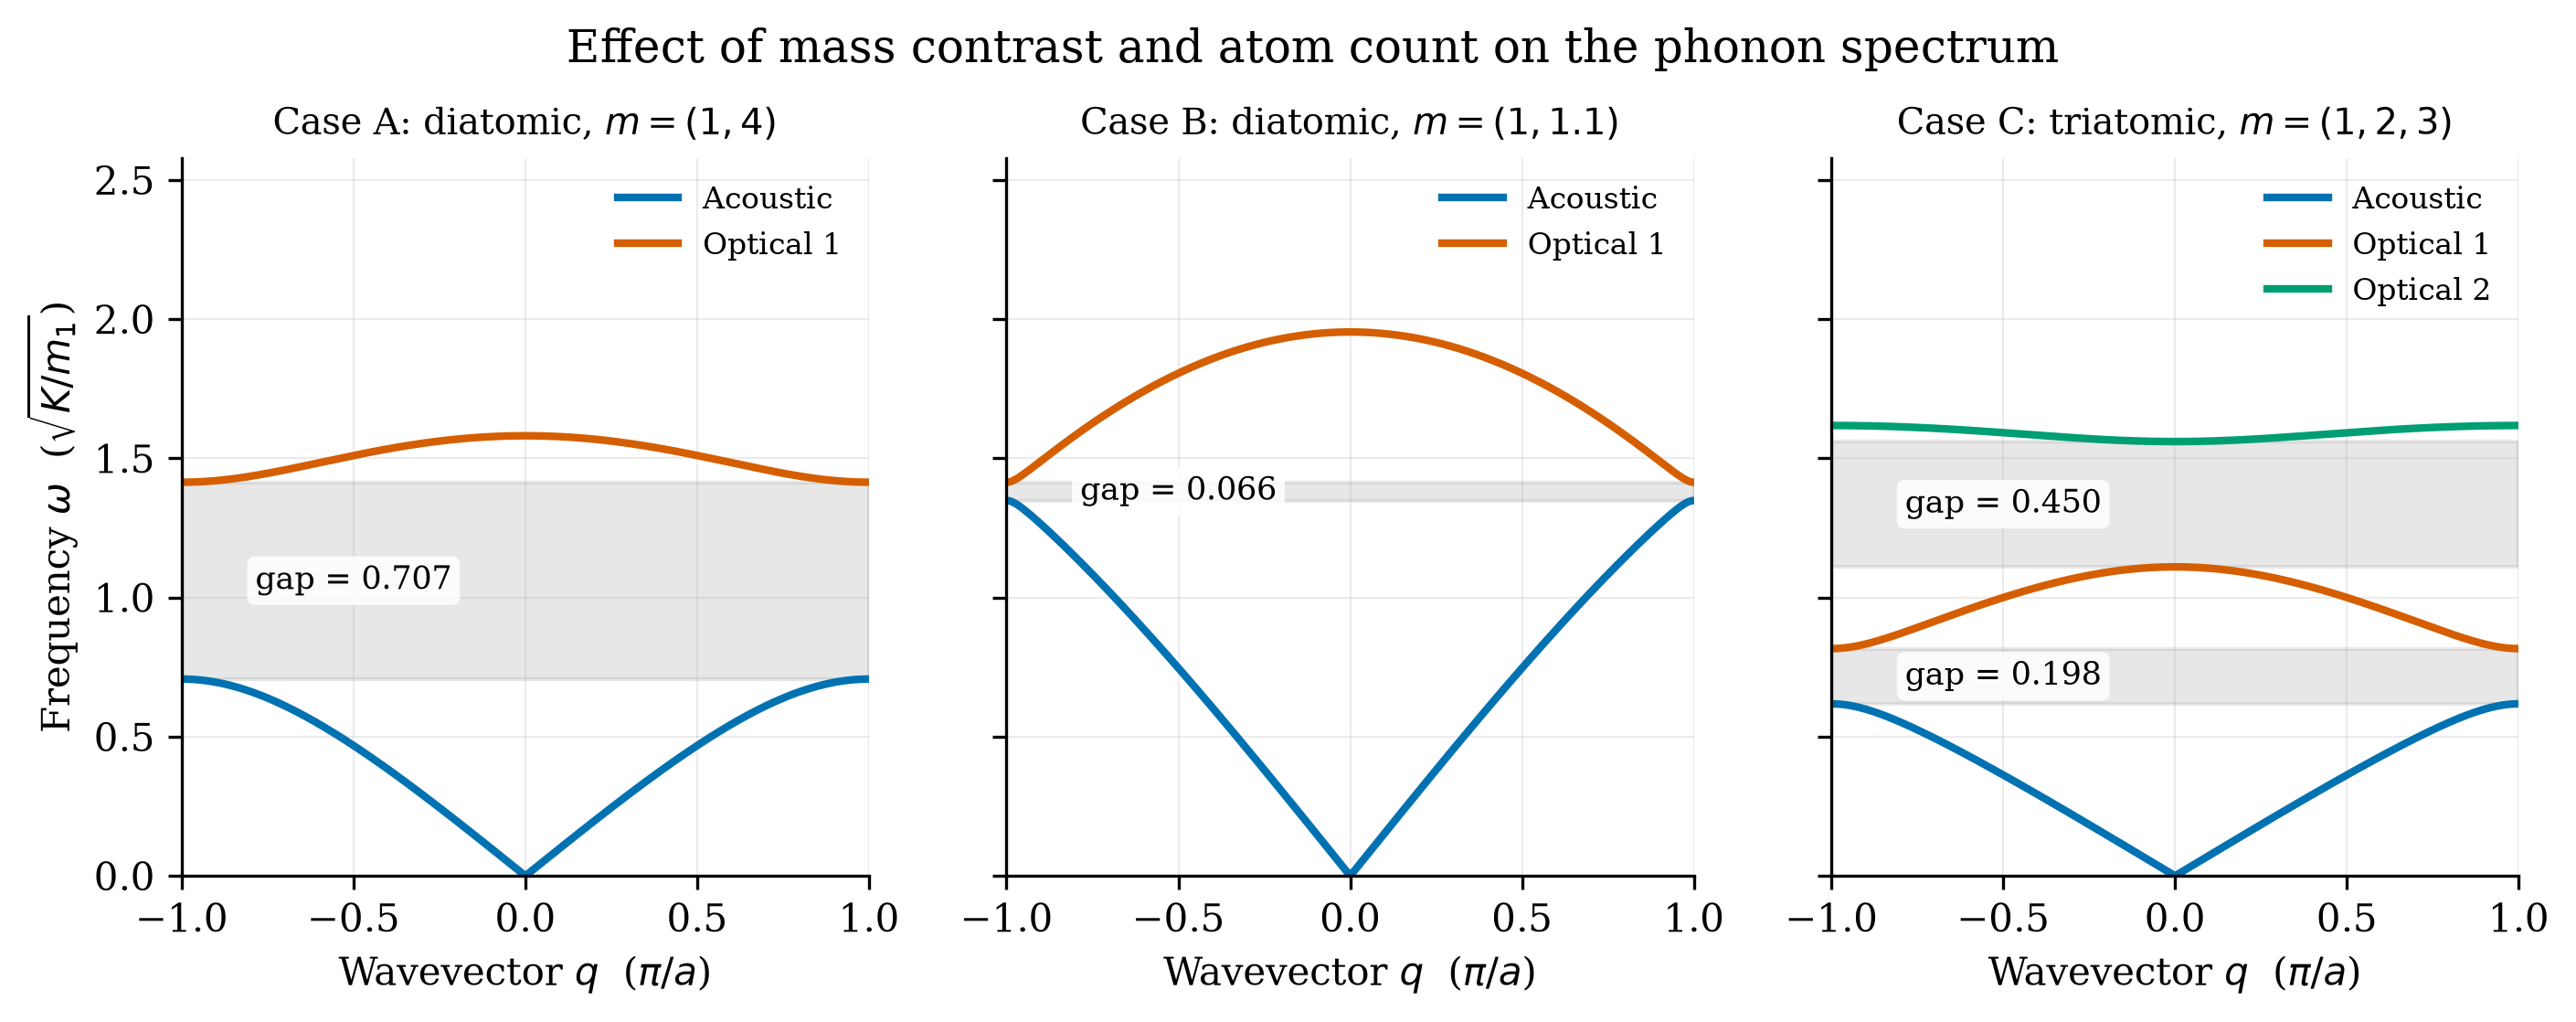
\includegraphics[width=\textwidth]{comparison.png}
\caption{Dispersion for the three cases on a common frequency scale. Shaded bands are forbidden
frequency ranges. The acoustic branch starts linearly from the origin in all three.}
\label{fig:comparison}
\end{figure*}

\begin{table*}[t]
\centering
\small
\begin{tabular}{llrrrr}
\toprule
\textbf{Case} & \textbf{Masses} & \textbf{Acoustic max} & \textbf{Optical range} & \textbf{Gap(s)} & $v_s$ \\
\midrule
A & $(1,4)$     & 0.7071 & 1.4142--1.5811 & 0.7071 & 0.3162 \\
B & $(1,1.1)$   & 1.3484 & 1.4142--1.9540 & 0.0658 & 0.4880 \\
C & $(1,2,3)$   & 0.6180 & 0.8165--1.1101, 1.5602--1.6180 & 0.1985, 0.4501 & 0.2357 \\
\bottomrule
\end{tabular}
\caption{Computed branch limits, gaps and sound velocities, in units of $\sqrt{K/m_1}$.}
\label{tab:cases}
\end{table*}

\subsection{Case A --- strong mass contrast}
\label{sec:caseA}

With $m_2/m_1 = 4$ the spectrum splits cleanly. The acoustic branch tops out at
$\omega = 0.7071 = \sqrt{2K/m_2}$ and the optical branch bottoms at
$\omega = 1.4142 = \sqrt{2K/m_1}$, both at the zone boundary and both matching the analytic zone-edge
values exactly. The gap of $0.7071$ is wide --- it spans half the entire frequency range of the
crystal. Physically, at the zone edge the two sublattices decouple: in the acoustic mode only the
heavy atoms move appreciably, in the optical mode only the light ones, so each frequency is that
of a single mass on its springs.

\subsection{Case B --- near-equal masses}

Raising $m_2$ by only 10\% above $m_1$ leaves a gap of $0.0658$, barely a tenth of Case A's. The
two branches very nearly join at the zone boundary, and the spectrum approaches the single
folded branch of a monatomic chain. This is the diagnostic case: the gap is a consequence of the
\emph{two-member basis}, and it closes continuously as that basis becomes trivial, rather than
being an independent property of the lattice. Figure~\ref{fig:gap} traces this directly.

\begin{figure}[h]
\centering
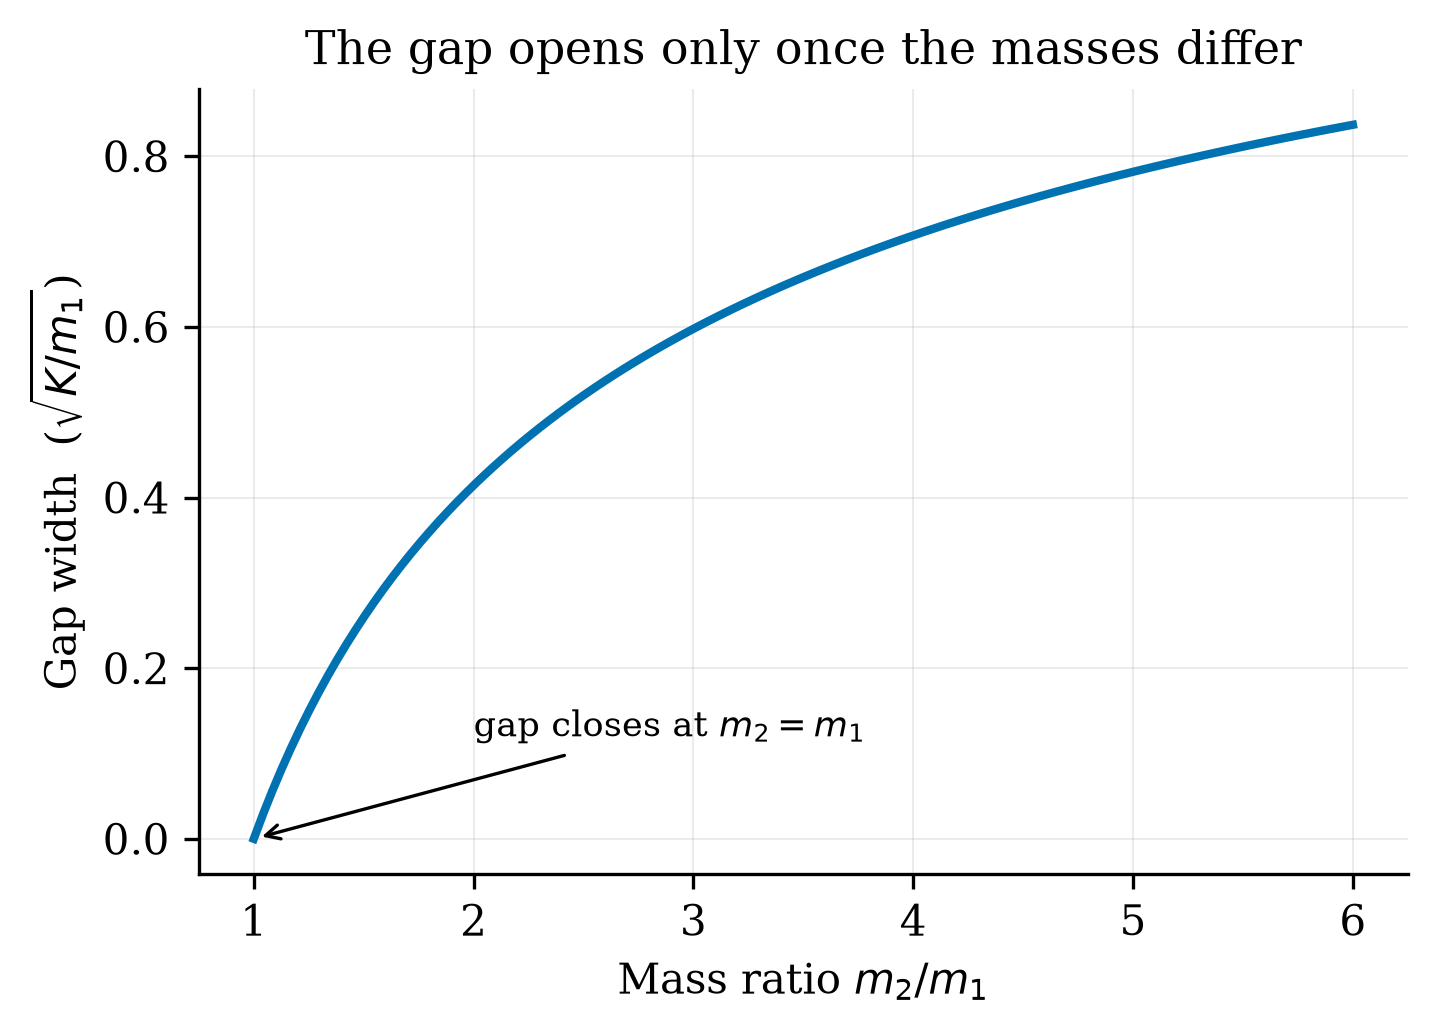
\includegraphics[width=\columnwidth]{gap_vs_ratio.png}
\caption{Gap width against mass ratio for a diatomic chain. The gap grows monotonically from zero
at $m_2 = m_1$; there is no threshold ratio below which a gap fails to appear.}
\label{fig:gap}
\end{figure}

\subsection{Case C --- three atoms per cell}

With $p=3$ there are one acoustic and two optical branches, and correspondingly two gaps,
$0.1985$ and $0.4501$. The general rule is visible here: $p$ atoms per cell give $p$ branches and
up to $p-1$ gaps. The upper optical branch is noticeably flat, varying only between $1.5602$ and
$1.6180$ across the whole zone. A flat branch means a near-zero group velocity
$\partial\omega/\partial q$: those modes carry almost no energy through the crystal, and they
appear in the density of states as a sharp peak.

\subsection{Effect of the spring constant}

\begin{figure*}[t]
\centering
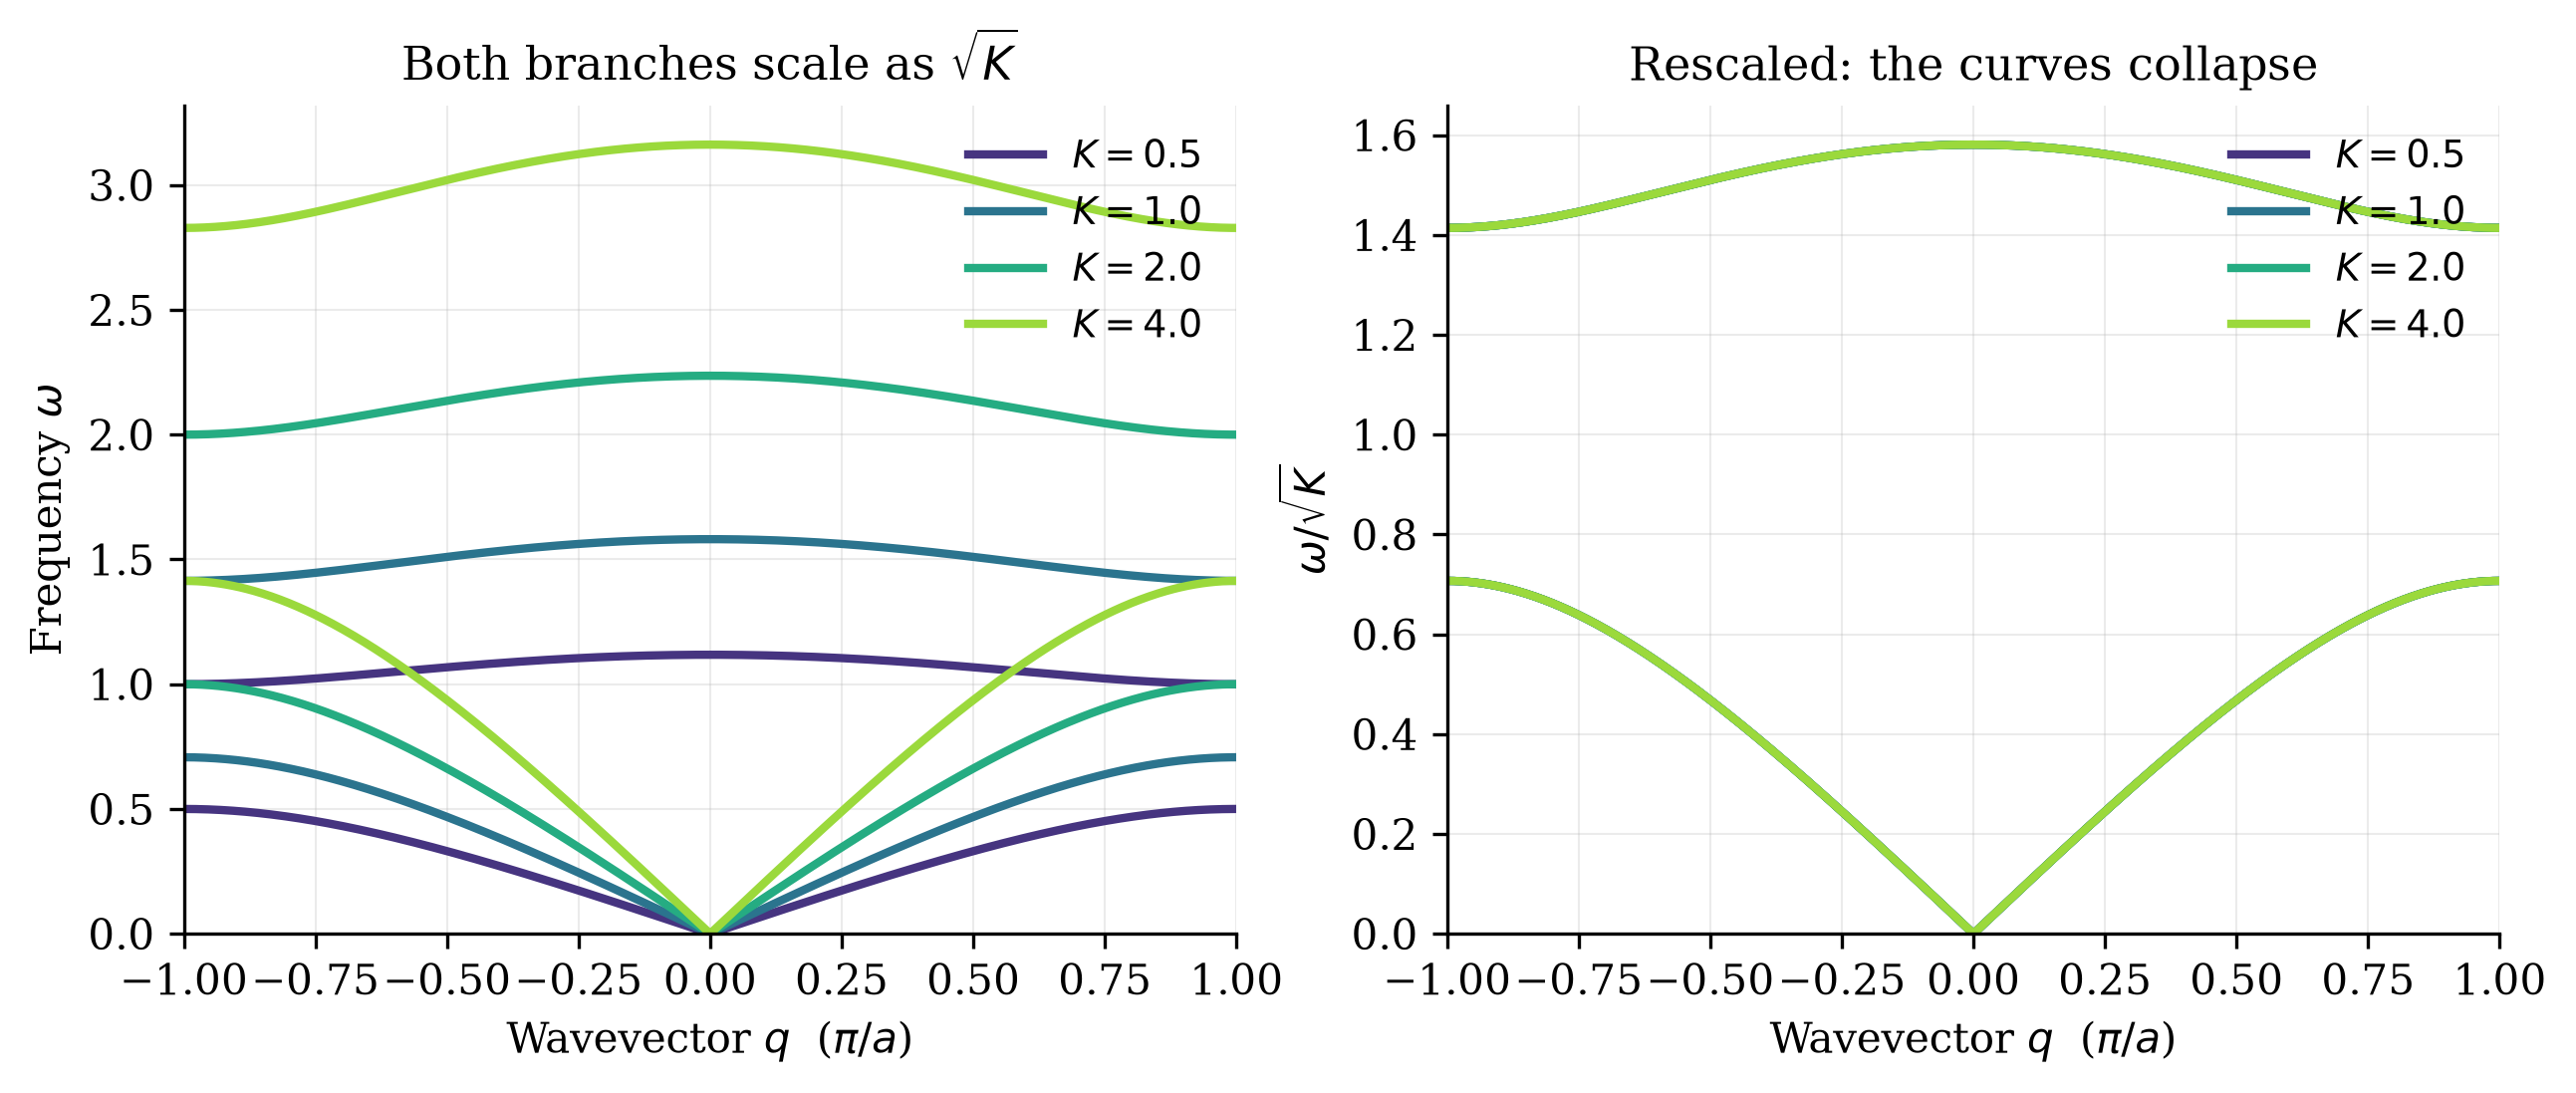
\includegraphics[width=\textwidth]{spring_sweep.png}
\caption{Left: Case A dispersion at four spring constants. Right: the same curves divided by
$\sqrt{K}$, collapsing onto a single pair.}
\label{fig:spring}
\end{figure*}

The spring constant enters \eqref{eq:Ddiag}--\eqref{eq:Dinter} as an overall multiplier, so
$D(q) \propto K$ and therefore $\omega \propto \sqrt{K}$ at every $q$. Figure~\ref{fig:spring}
confirms this: rescaling by $\sqrt{K}$ collapses all four spectra onto one curve. Stiffer springs
raise every frequency, including the gap width in absolute terms, but leave the \emph{shape} of
the spectrum --- and hence all ratios, including gap-to-bandwidth --- untouched. Mass contrast
and spring constant therefore play different roles: masses set the structure of the spectrum,
$K$ sets only its scale.

\subsection{Density of states}

\begin{figure*}[t]
\centering
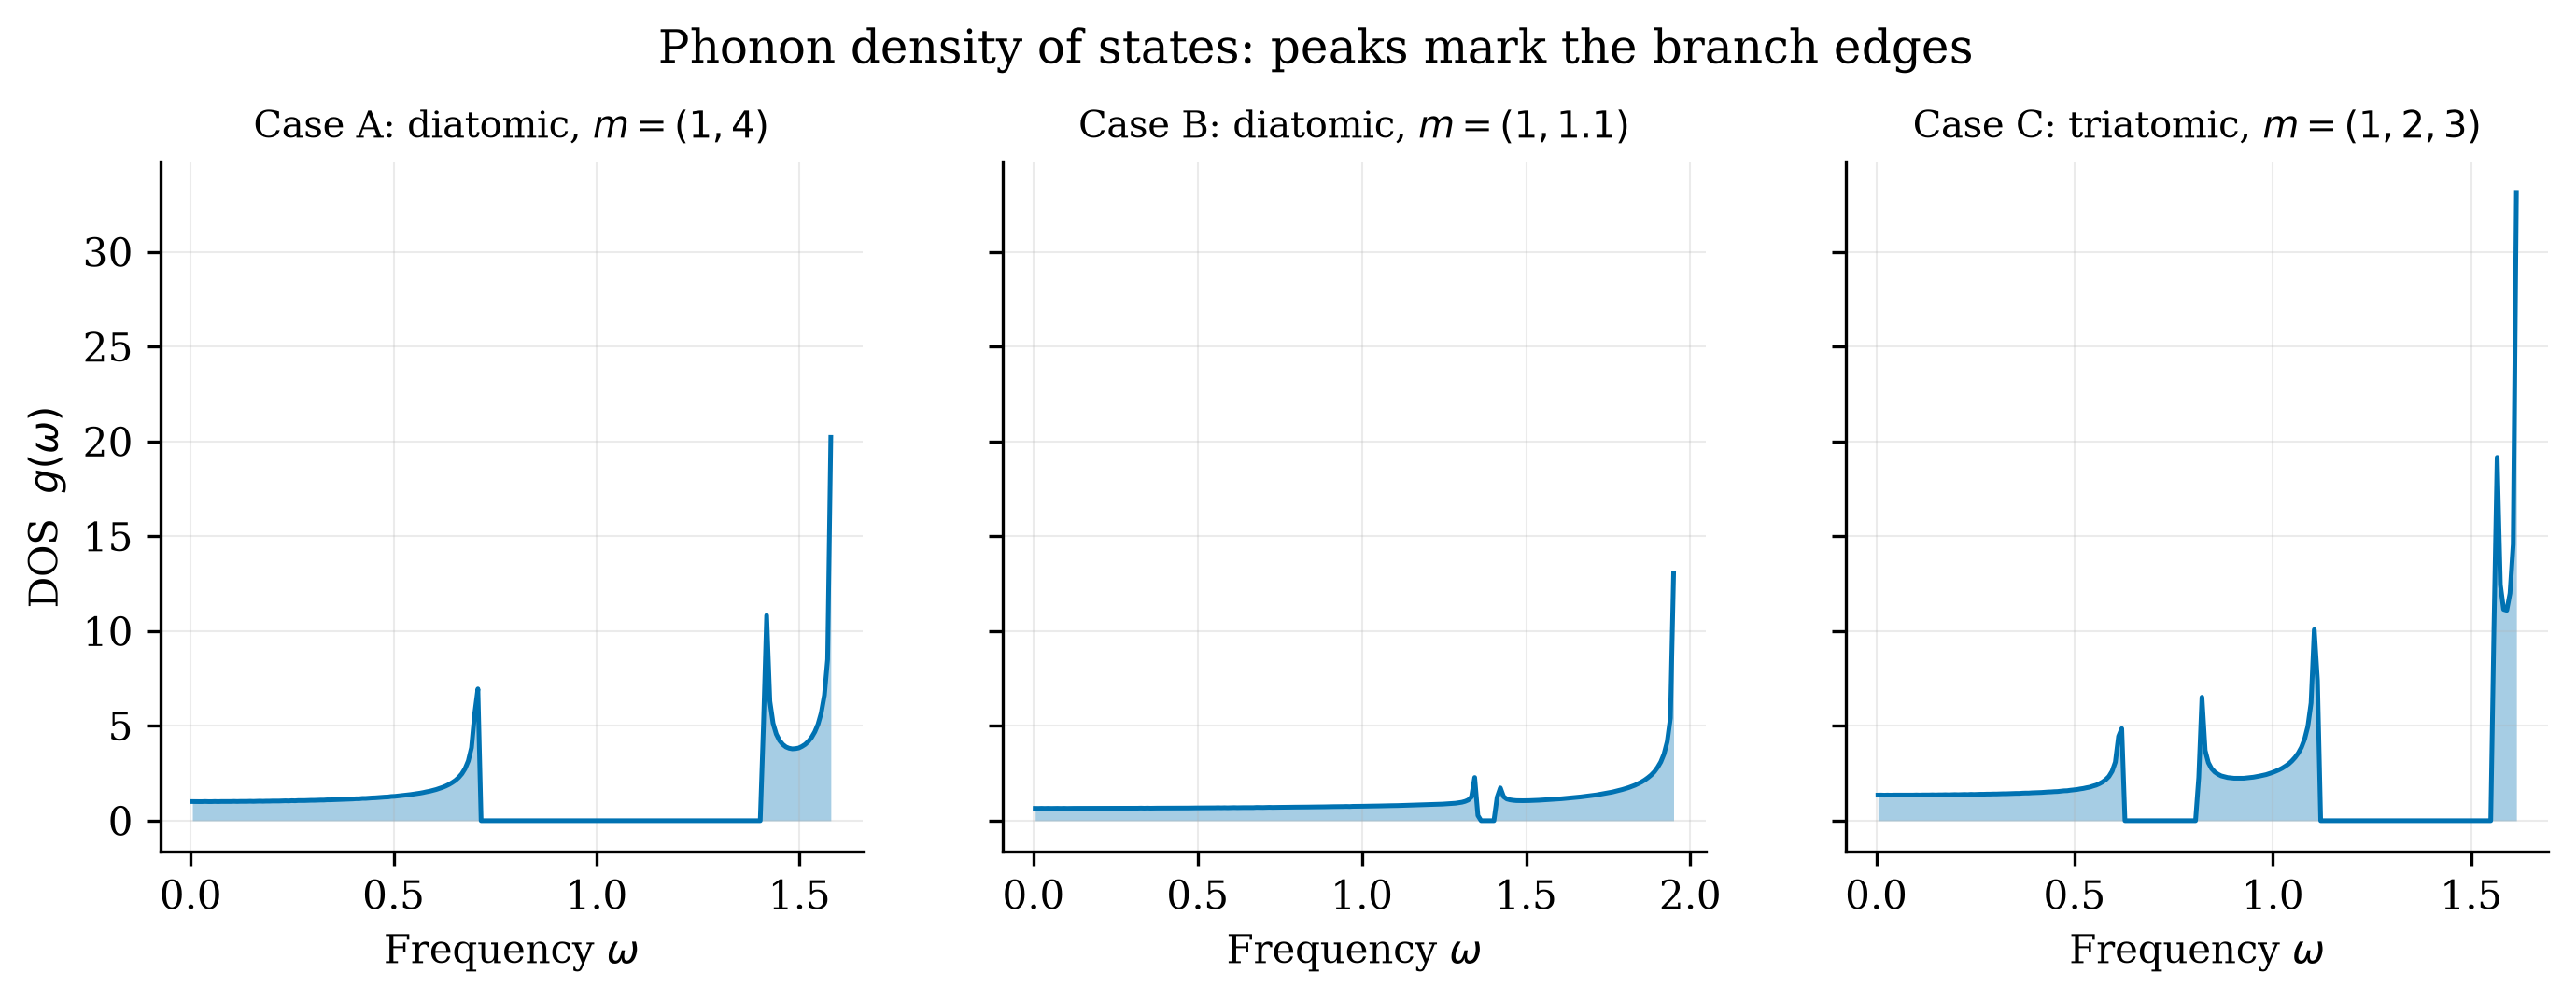
\includegraphics[width=\textwidth]{dos.png}
\caption{Phonon density of states for the three cases, from a histogram of $\omega$ over a dense
$q$ mesh. Empty regions are the bandgaps of Table~\ref{tab:cases}.}
\label{fig:dos}
\end{figure*}

The density of states $g(\omega)$ counts modes per unit frequency. It is zero inside every gap,
which is what "forbidden frequency range" means in practice: an incident wave at such a frequency
finds no mode to propagate in and is reflected. The sharp peaks are van Hove singularities,
occurring where a branch has zero slope --- at the zone centre and boundary, and across the whole
of a flat branch. Case C's flat upper optical branch produces the most pronounced peak of the
three, exactly as its shape in Figure~\ref{fig:comparison} predicts.

\subsection{Eigenfrequencies and their significance}

\begin{table}[h]
\centering
\small
\begin{tabular}{llrr}
\toprule
\textbf{Case} & \textbf{Branch} & $\omega$ at $q=0$ & $\omega$ at $q=\pi/a$ \\
\midrule
A & Acoustic  & 0.0000 & 0.7071 \\
  & Optical 1 & 1.5811 & 1.4142 \\
\midrule
B & Acoustic  & 0.0000 & 1.3484 \\
  & Optical 1 & 1.9540 & 1.4142 \\
\midrule
C & Acoustic  & 0.0000 & 0.6180 \\
  & Optical 1 & 1.1101 & 0.8165 \\
  & Optical 2 & 1.5602 & 1.6180 \\
\bottomrule
\end{tabular}
\caption{Eigenfrequencies at the zone centre and zone boundary.}
\label{tab:eigen}
\end{table}

\begin{figure*}[t]
\centering
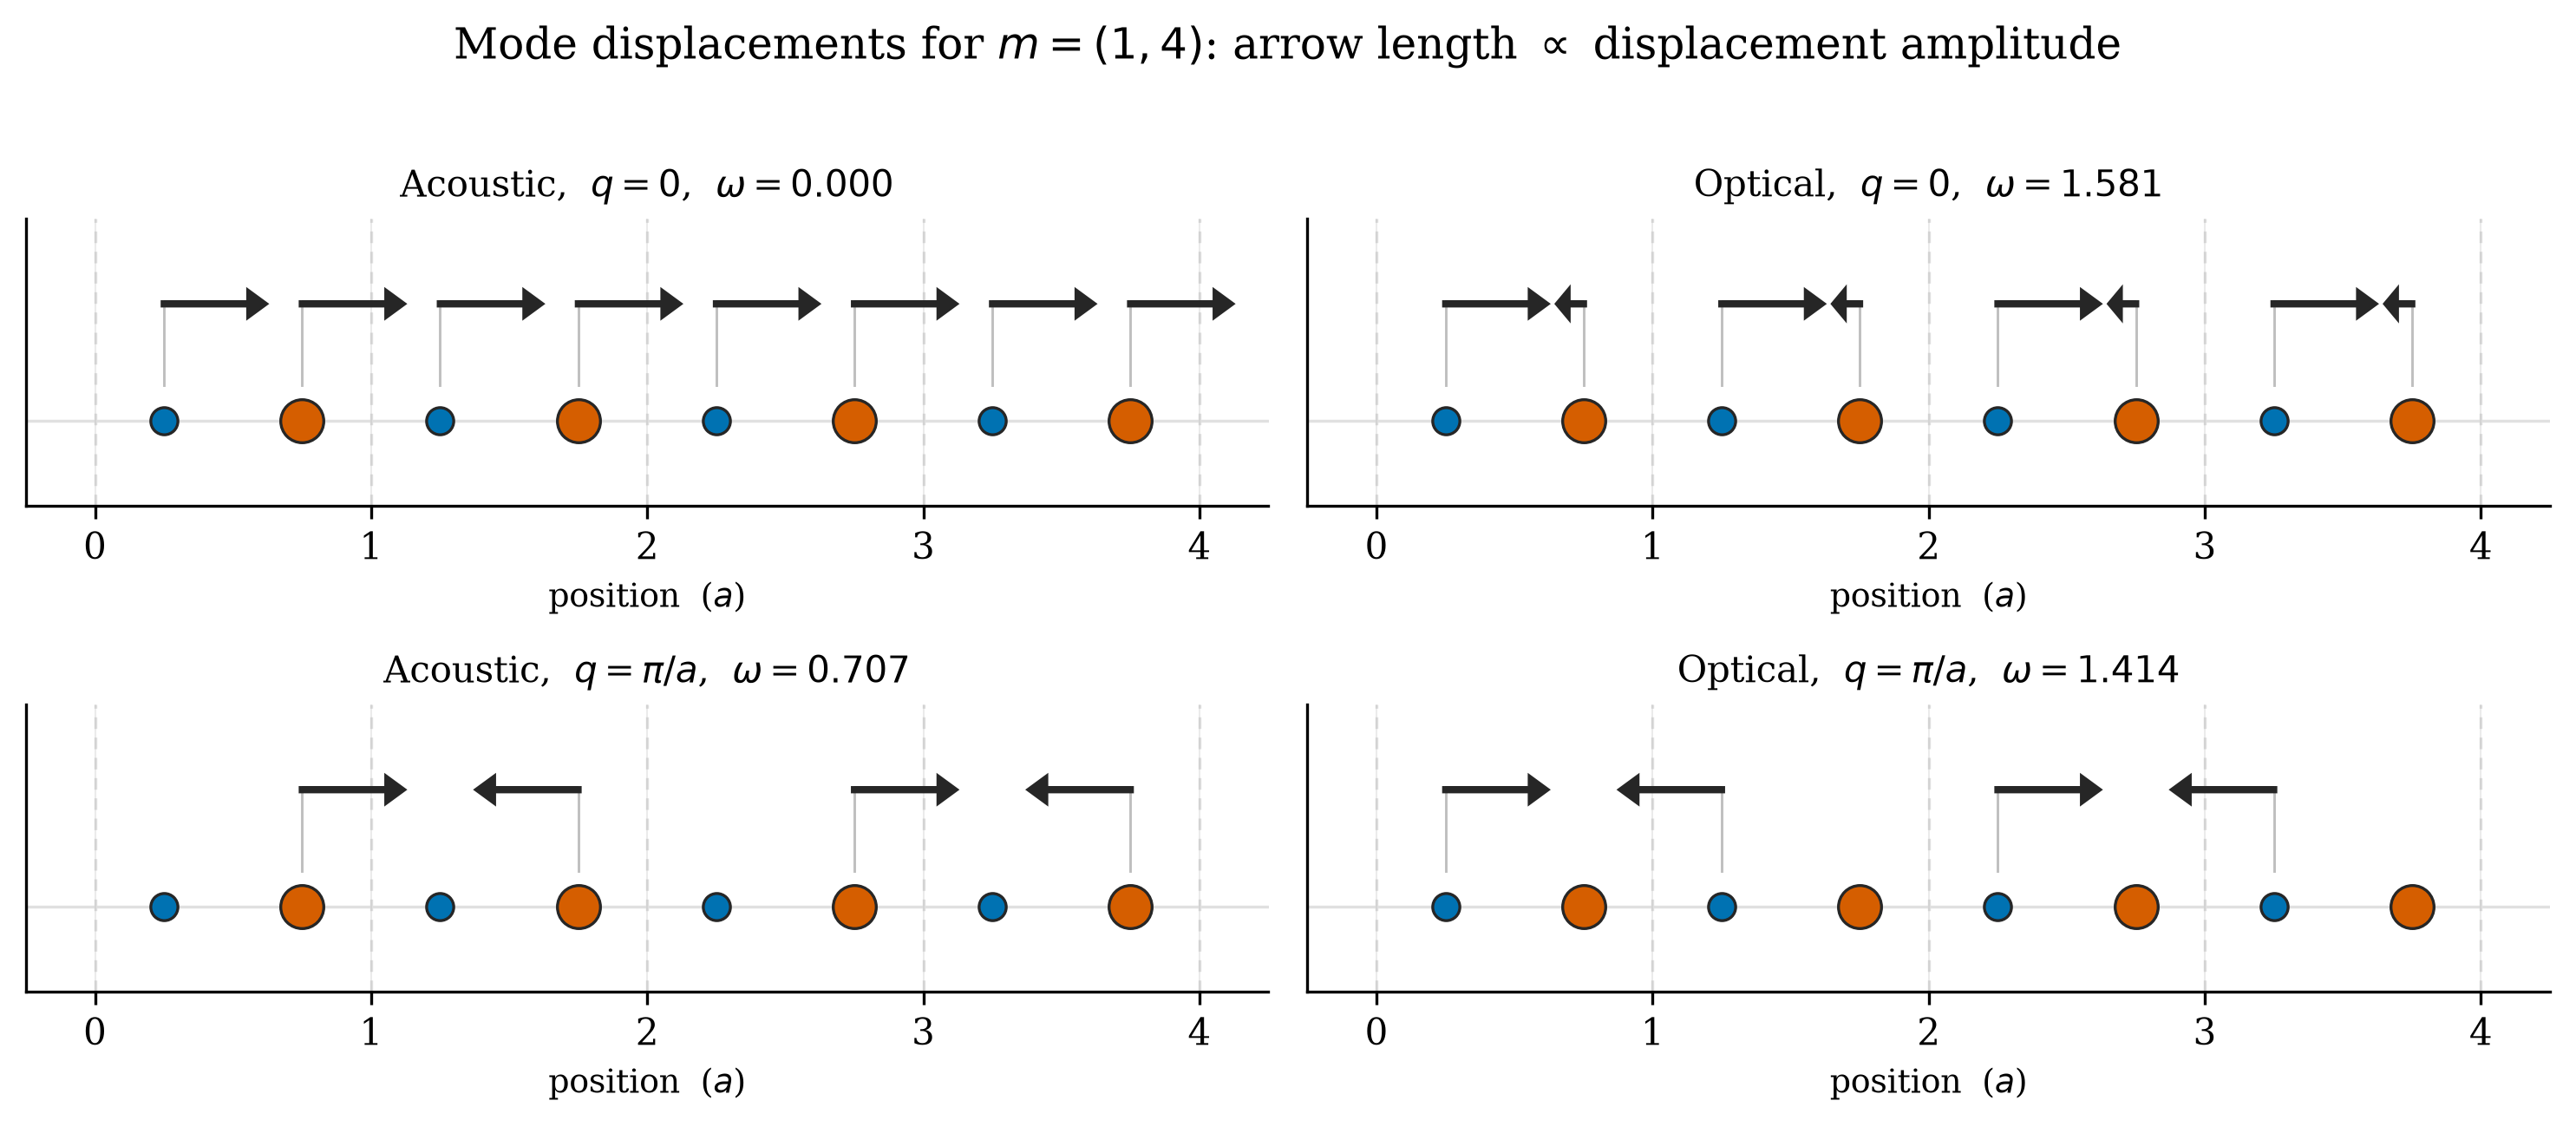
\includegraphics[width=\textwidth]{modes.png}
\caption{Displacement patterns of the two branches of the $m=(1,4)$ chain. Arrows show the
\emph{physical} displacement amplitudes $u_j = e_j/\sqrt{m_j}$, not the mass-weighted
eigenvector components $e_j$ returned by the solver; this is why the light atom swings four
times as far as the heavy one in the optical mode at $q=0$, keeping $\sum_j m_j u_j = 0$ so the
cell's centre of mass stays at rest. Small circles are the light atoms, large circles the heavy
ones. At $q=0$ the acoustic mode translates every atom equally. At $q=\pi/a$ the two sublattices
decouple completely --- the eigenvectors are exactly $(0,1)$ and $(1,0)$ --- so half the atoms
carry no arrow at all, and the moving ones reverse from cell to cell through the factor
$e^{iqna}=(-1)^n$.}
\label{fig:modes}
\end{figure*}

The eigenfrequencies are the natural frequencies of the lattice: a mode excited at $\omega_i(q)$
oscillates indefinitely at that frequency in the harmonic approximation, and any arbitrary motion
of the chain decomposes into a superposition of them. Table~\ref{tab:eigen} shows the two limiting
cases.

At $q = 0$ all cells move identically. The acoustic eigenvalue is exactly zero in every case,
since translating the whole crystal stretches no spring. The optical frequencies there are
nonzero because the atoms inside a cell move against each other --- for Case A, $1.5811 =
\sqrt{2K(1/m_1 + 1/m_2)}$, the frequency of two masses vibrating on a shared spring about their
common centre of mass. This is the mode that couples to infrared light in a real ionic crystal,
and the origin of the name "optical".

At $q = \pi/a$ adjacent cells move in antiphase, the shortest wavelength the lattice supports.
Both branches flatten here, which is why the gap edges in Table~\ref{tab:cases} are attained at
the boundary. Figure~\ref{fig:modes} shows the eigenvectors directly, and makes the decoupling
of Sec.~\ref{sec:caseA} explicit: at the zone edge the acoustic eigenvector is $(0,1)$ and the
optical one $(1,0)$, so each branch is a single sublattice vibrating while the other stands
still.

\section{Conclusions}

Reducing the chain's equations of motion to a $p \times p$ Hermitian eigenvalue problem gives a
method that handles any number of atoms per cell with no change of algorithm, and reproduces the
textbook monatomic and diatomic solutions to within $10^{-13}$. Applying it:

\begin{itemize}
  \item $p$ atoms per unit cell give one acoustic and $p-1$ optical branches, with up to $p-1$
        gaps between them.
  \item The bandgap is produced by mass contrast within the cell and closes continuously as the
        masses are equalised --- $0.7071$ at a mass ratio of 4, $0.0658$ at a ratio of 1.1, zero
        at 1.
  \item The spring constant scales all frequencies as $\sqrt{K}$ and changes nothing else about
        the spectrum.
  \item Flat branches produce van Hove peaks in the density of states and carry negligible group
        velocity.
\end{itemize}

The obvious limitations are the harmonic approximation, which excludes thermal expansion and
phonon lifetimes, and the restriction to nearest-neighbour coupling in one dimension.

\section*{Reproducing this work}

\begin{verbatim}
uv venv --python 3.12 .venv
uv pip install numpy scipy matplotlib \
     streamlit pandas
cd question_3
python test_phonon.py    # checks
python make_figures.py   # figures
streamlit run app.py     # interface
\end{verbatim}

\onecolumngrid
\appendix

\section{Complete source code}

All listings are included directly from the source files, so they cannot drift from the code that
produced the results above. The files are, in dependency order: the physics core, its validation
suite, the shared plotting style, the figure generator, and the interactive interface.

\subsection{\texttt{phonon.py} --- physics core}
\lstinputlisting{../phonon.py}

\subsection{\texttt{test\_phonon.py} --- validation suite}
\lstinputlisting{../test_phonon.py}

\subsection{\texttt{common/style.py} --- shared plotting style}
\lstinputlisting{../../common/style.py}

\subsection{\texttt{make\_figures.py} --- figure generation}
\lstinputlisting{../make_figures.py}

\subsection{\texttt{app.py} --- interactive interface}
\lstinputlisting{../app.py}

\twocolumngrid

\begin{thebibliography}{9}
\bibitem{kittel} C.~Kittel, \textit{Introduction to Solid State Physics}, 8th ed., Wiley, 2005.
  Chapter 4, lattice vibrations and the diatomic chain.
\bibitem{ashcroft} N.~W.~Ashcroft and N.~D.~Mermin, \textit{Solid State Physics},
  Holt--Saunders, 1976. Chapters 22--23, the harmonic crystal.
\bibitem{dove} M.~T.~Dove, \textit{Introduction to Lattice Dynamics}, Cambridge University
  Press, 1993.
\bibitem{tong} D.~Tong, \textit{Lectures on Solid State Physics}, University of Cambridge.
  \url{https://www.damtp.cam.ac.uk/user/tong/aqm.html}
\bibitem{numpy} C.~R.~Harris \textit{et al.}, ``Array programming with NumPy'',
  \textit{Nature} \textbf{585}, 357--362 (2020). \texttt{numpy.linalg.eigvalsh} documentation.
\bibitem{matplotlib} J.~D.~Hunter, ``Matplotlib: A 2D graphics environment'',
  \textit{Computing in Science \& Engineering} \textbf{9}, 90--95 (2007).
\bibitem{streamlit} Streamlit documentation. \url{https://docs.streamlit.io}
\end{thebibliography}

\end{document}
